\textbf{A previous version of this chapter was published in \cite{CharltonSana2023SimWrapper}.}

\hypertarget{simwrapper-introduction}{%
\section{Introduction}
\label{simwrapper-introduction}}

In Part 1, the technological foundation was set for building data visualization portals. Then in Part 2, the components of that foundation were combined and reformulated to produce three bespoke project websites, each of which was built to support analysis, decisionmaking, and public knowledge transfer. The idea of building a long string of separate, purpose-built websites over and over again seemed like an overly duplicative approach: much of the infrastructure and the code itself was essentially just being copied from one site to the next. Having confirmed the utility and capabilities of a fully browser-based data visualization approach for three individual project portals, it was time to find a way to generalize the method in an extensible and scalable way.

An entirely generic data visualization platform is inherently more challenging to create than a project portal, as every researcher investigates widely disparate questions and is focused on completely different outputs. One researcher may be using EpiSim to explore pandemic simulations, while another uses MATSim to predict future demand-responsive shared taxi vehicle flows, while a third is performing emergency-response evacuation planning, or emissions reduction through increased transit ridership efforts. The tool needs to be extremely flexible without foreknowledge of the precise questions that will be asked.

This chapter describes \textbf{SimWrapper}, an open-source web-based data visualization platform that was developed with the goal that it be useful for anyone working with MATSim outputs, and ultimately for other data-intensive transport microsimulation models as well.

% ------------------------------------------------------------------------------------
% ## SimWrapper in a Nutshell
% ------------------------------------------------------------------------------------

\hypertarget{simwrapper-overview}{%
\section{Overview: SimWrapper, in a nutshell}
\label{simwrapper-overview}}

The success of the projects described in Part 2 meant that many design questions were already settled before work began on SimWrapper. SimWrapper would be an extension of the ideas embedded in those projects: simple file-based storage of simulation results, accessed from a front-end website with multiple visualization components for different types of data views, all configured with a simple text-based descriptive configuration language that requires zero JavaScript coding on the part of project analysts.

SimWrapper, in a nutshell:

\begin{itemize}
\item
    is a static website that runs client-side JavaScript in the form of
    a single page application (\gls{SPA}), a common approach in modern web
    development that is compatible with all recent web browsers;
\item
    supports network-based file storage for public- and/or
    group-accessible shared data files (model runs), but has no other
    back-end server requirements and can run completely locally if no
    network file storage is available or needed;
\item
    allows the user to navigate through their local filesystem or shared
    network storage of model runs to view results that are saved in a
    specific folder, rather than a database-centric approach. This
    matches the design of MATSim and other simulation models which
    produce collections of output files by default;
\item
    provides a collection of data visualization archetypes that are each
    appropriate for displaying a certain type of data, for example
    various statistical chart types (bars, lines, area, pie), geographic
    data viewers supporting road and transit network link data, area
    aggregation (``choropleth'' and ``spider'') maps, XY coordinate
    plots, and many more;
\item
    can combine all of these disparate components into cohesive
    dashboards that the user can lay out in a flexible manner, using
    small declarative configuration files. These configurations can be
    applied across multiple projects or simulation runs;
\item
    is GDPR (General Data Protection Requirement) compliant. The website performs
    no user tracking, has no centralized data storage,
    no advertising, nor any other privacy-compromising misfeatures.
    SimWrapper is not a product for sale; it is an open research platform.
\end{itemize}

The following sections explore design aspects of SimWrapper in more detail.

\hypertarget{simwrapper-components}{%
\section{SimWrapper platform architecture}
\label{simwrapper-components}}

Figure \ref{fig:simwrapper-flowchart-1} shows a simplified depiction of the SimWrapper platform architecture. The code is organized as a \gls{SPA} which runs entirely inside the user's web browser. The site then accesses files stored either locally or on a network server (such as on the Internet or a local file server).

\begin{figure}[ht]
  \centering
  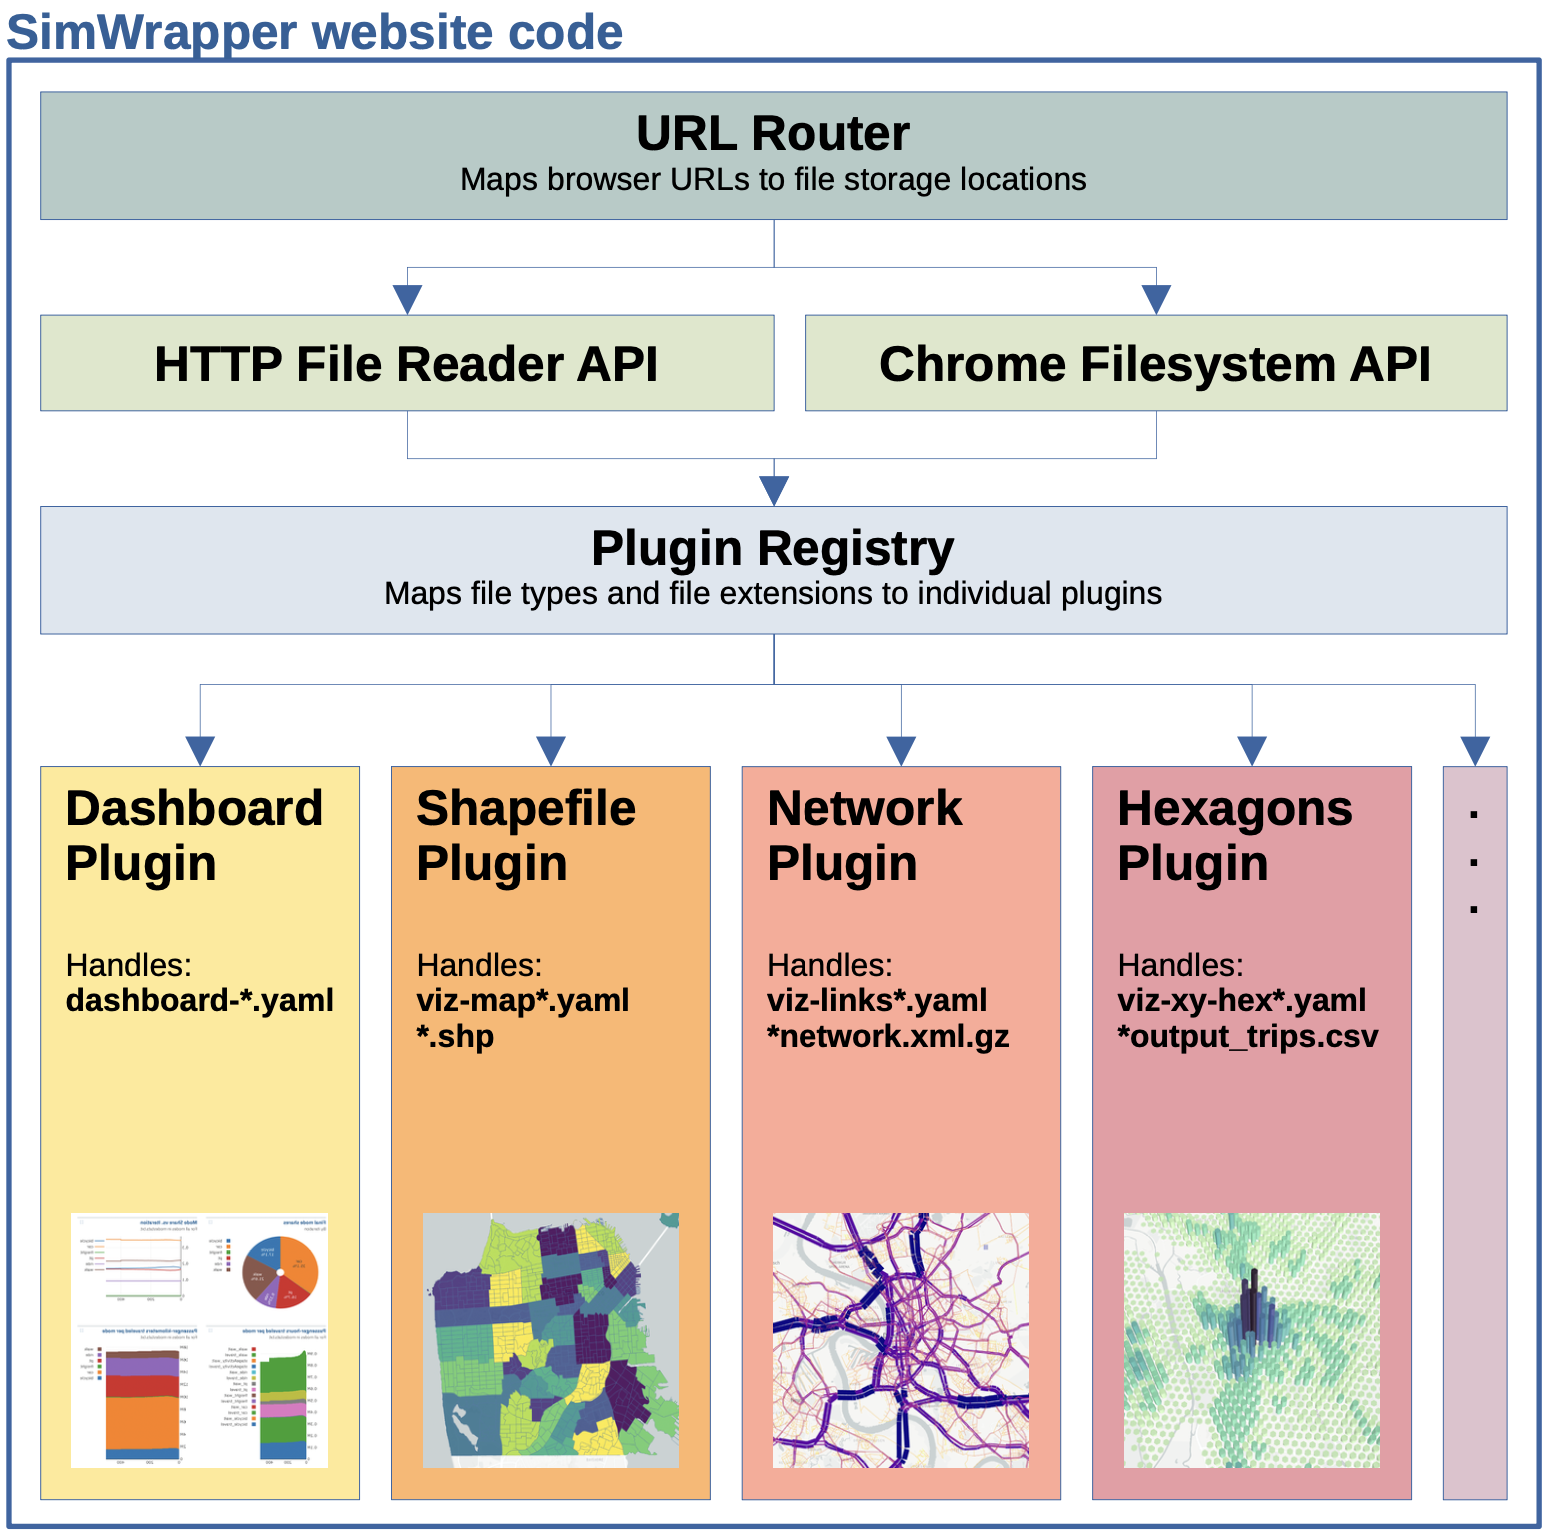
\includegraphics[width=0.95\linewidth]{chapters/31-simwrapper/images/flowchart-1.png}
  \caption{SimWrapper platform architecture. This shows the organization and flow of the client JavaScript code.}
  \label{fig:simwrapper-flowchart-1}
\end{figure}

The main point of entry in the application is the URL router, which maps the URL specified in the web browser to a specific file storage location. Any installation of SimWrapper can define URL endpoints; for example, at \gls{VSP} there are multiple folders on the departmental file server which are designated as SimWrapper file storage locations. One is for general MATSim outputs; others are for specific project outputs (see c.f. Chapter \ref{ch:simwrapper-sites} for further examples).

The router passes the file location to code which can fetch the file resource. Currently two such file services are enabled, the HTTP file system that can access any publicly accessible web server, and a local file access service that uses an advanced API available on Google Chrome to enable local file access (see section \ref{simwrapper-special-case-chrome-and-the-file-system-access-api} for more detail).

Files are passed to specific visualization plugins using the \emph{plugin registry}. Every SimWrapper plugin defines a set of filename patterns that it can handle, e.g. the shapefile plugin can read \texttt{.SHP} shapefiles and the MATSim network link viewer can read MATSim \texttt{network.xml.gz} files. The plugins also register which YAML configuration files they can read: the YAML configuration filenames match a specific pattern, e.g. the network link viewer will open \texttt{viz-links-....yaml} files. Documentation for each SimWrapper plugin enumerates the types and filenames of the files that those plugins can read.

What happens next is up to the plugin: the shapefile or network is read, the configuration details are used to set up dashboard layouts, display and data information is processed, titles are set, and so on.

Figure \ref{fig:simwrapper-flowchart-2} lists some typical file types that might be found in SimWrapper storage locations. Simulation outputs are often saved in one folder per simulation, named in such a way that analysts can easily find their outputs in a hierarchical file system.

One special folder name is reserved: if a folder named \texttt{.simwrapper} is present, the configuration files within that folder will be applied to all child folders and sibling folders adjacent to it: in this manner, project-wide configurations, dashboards, and settings can be defined in one location and applied to many simulation outputs automatically.

\begin{figure}[ht]
  \centering
  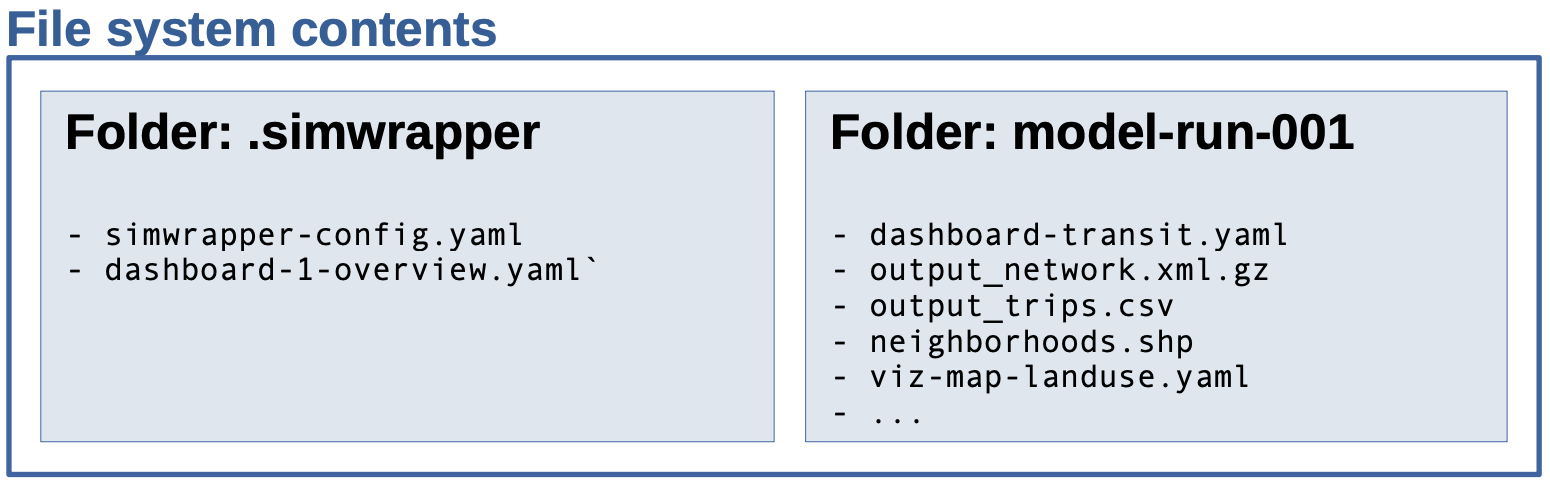
\includegraphics[width=0.95\linewidth]{chapters/31-simwrapper/images/flowchart-2.png}
  \caption{Some typical SimWrapper configuration files and simulation output files. Configuration files in the \texttt{.simwrapper} folder are applied to every sibling folder, allowing centralized project-level configuration.}
  \label{fig:simwrapper-flowchart-2}
\end{figure}

With the URL router, file storage, and visualization plugin components in place, the architecture is essentially complete: the browser code associates a user-specified URL to a specific folder or file in the defined file storage area; that file is read and the contents are passed to a specific visualization plugin based on its name or contents; and the plugin then has everything it needs to create the requested visualization.

Every visualization plugin is not discussed in depth here, but see Appendix \ref{appendix:simwrapper} for a more exhaustive list. Some of the details are worth exploring, and are described next.

% ------------------------------------------------------------------------------------

\hypertarget{simwrapper-javascript-libraries}{%
\section{JavaScript component libraries}\label{simwrapper-javascript-libraries}}

The starting point for SimWrapper was the PAVE project website described in \ref{ch:pave}. This involved selecting a curated set of JavaScript infrastructure libraries for common needs, and then writing bespoke code for our specific use case and for the ``glue'' between the components.

The experience with PAVE led to selection of existing JavaScript libraries for the following; all of the libraries mentioned below are open source and available on the NPM software registry\footnote{NPM is available online at \url{https://npmjs.org}}.

\begin{itemize}
\item
  User interface interaction: the \emph{Vue} framework is the primary glue that
  links JavaScript code to the page layout, calling specific functions for user
  interactions such as mouse clicks and other user-initiated events.
\item
  Data loading: Most MATSim outputs are either tabular text files in CSV
  format, or compressed XML files with explicit schemas. The \emph{Papaparse}
  and \emph{Fast-XML-Parser} libraries handle loading these two data formats.
\item
  Charting: the PAVE site included statistical charts such as bar, line,
  pie, and scatter plots, and used the \emph{Plotly} JavaScript library. Plotly
  is very easy to use and covers most standard cartesian plot types (bars, areas, lines, scatterplots) and offers some advanced non-cartesian plot types as well.
\item
  Geographic data on maps: initial efforts using the \emph{Mapbox}
  JavaScript library were unsatisfactory and led to use of the more performant
  \emph{Deck.gl} collection of \gls{GPU}-based visualizations.
\item
  Animation: the agent-based animations for COVID-Sim used the \emph{Three.js}
  3D animation library.
  \item
  Filtering: fast filtering of large datasets is performed by the \emph{crossfilter} package.
\end{itemize}

All of these libraries share compatible open-source licenses, and are embedded in SimWrapper under the terms of those licenses.

% ------------------------------------------------------------------------------------
% ## Modifications needed for a generic tool
% ------------------------------------------------------------------------------------

\hypertarget{simwrapper-modifications-necessary}{%
\section{Iterative improvements to the platform during development}
\label{simwrapper-modifications-necessary}}

User feedback from the previous projects (see sections \ref{avov-results} and \ref{pave-feedback}), as well as from internal staff during the course of development, helped direct changes and improvements for the generic tool. In summary, changes were needed in the following categories:

\begin{itemize}
\item
  Performance. The network link viewer in particular was slow to load
  datasets for large simulations. This was not a problem for AVÖV
  because the study areas were less populated, but for PAVE, many
  of the datasets for the Berlin simulation area were nonperformant.
\item
  Flexibility. Each of the data visualization components needed to be
  made much more flexible. For example, the PAVE link viewer assumed
  that input data was specified by time period, whereas a generic tool
  needs to depict any sort of data.
\item
  Output traversal. While PAVE had a hard-coded set of alternatives that
  could be browsed in a simple manner, a generic tool needs some sort of
  scenario selection and/or traversal capability; a way to browse the
  hierarchical file storage available.
\item
  Stability and resilience. The PAVE site included almost no error
  message reporting or helpful debugging infrastructure, because expert
  analysts carefully crafted the inputs for each alternative. A generic
  tool needs to be tolerant of user mistakes and helpful in guiding the
  user when inputs are lost or malformed.
\item
  Better defaults plus configurability. There is no illusion that this
  platform can replicate or replace a full-featured desktop application,
  of which there are many in the \gls{GIS} realm. Rather, users expressed a
  desire for a set of clear, curated defaults that have some
  configurability. For much more advanced configuration, a
  professionally-developed package such as QGis is likely more appropriate.
\end{itemize}

% ------------------------------------------------------------------------------------
% ## Accessing files via a Web Browser
% ------------------------------------------------------------------------------------

\hypertarget{simwrapper-accessing-files-through-a-web-browser}{%
\section{Accessing files through a web browser}
\label{simwrapper-accessing-files-through-a-web-browser}}

The use case of file storage via departmental file server is well-explored and very functional, as expressed in the project websites for COVID-Sim, AVOEV, and PAVE (see Part \ref{part:2projectsites}).

A key difference between those earlier project websites and SimWrapper is the need to ``meet the users where they are'' -- in other words, users may not have (or wish to use) a departmental file server with a public API endpoint serving data files. One of the primary feedback elements from the initial MatHub implementation described in Chapter \ref{ch:mathub} was that users found it too onerous to upload model run outputs to a second server system before being able to view or analyze anything. In addition to being wasteful of space (and MATSim outputs can be gigabytes in size!), it is time-consuming and generates user friction, discouraging use of the tool.

For regular users in the middle of their research workflow, something else is needed. Most internal users at VSP run simulations either on their personal laptop/desktop machines or on the university compute cluster, which has extensive attached storage but no public-facing access via the web. Furthermore, many runs often cannot be made public due to data security considerations, or may simply be of a transitory nature that precludes them being public.

Thus several alternative avenues for enabling users to view their outputs are described here.

% ------------------------------------------------------------------------------------
% ### How SimWrapper access files via HTTP
% ------------------------------------------------------------------------------------

\hypertarget{simwrapper-how-simwrapper-access-files-via-http}{%
\subsection{Serving files via HTTP}
\label{simwrapper-how-simwrapper-access-files-via-http}}

SimWrapper is designed to allow browsing of files from administrator-defined HTTP URLs, which represent the root locations of the file storage for that project. For example, the PAVE project datasets are all stored on the VSP public file server at the very long URL,

\href{https://svn.vsp.tu-berlin.de/repos/public-svn/matsim/scenarios/countries/de/berlin/projects/pave/website/}{svn.vsp.tu-berlin.de/repos/public-svn/matsim/scenarios/countries/de/berlin/projects/pave/website/}

That URL is the defined ``root'' of the project; all of the project dashboard configurations, model outputs, and processed data files exist in various subfolders subordinate to that location. The PAVE website at \href{https://vsp.berlin/pave/}{vsp.berlin/pave/} is set up to read files from that base URL.\footnote{But refer to section \ref{simwrapper-cors} for a discussion of CORS configuration, which is necessary to allow one website to read the files stored on another.}

SimWrapper elevates this to allow multiple configured root filesystems: the public VSP file server is one such root, but others can also be configured and are displayed on the home page of SimWrapper. Each root is expected to provide HTTP directory access to this storage: SimWrapper must be able to \emph{view directory listings} and \emph{retrieve file contents}. SimWrapper never writes any files anywhere; it is read-only.

% ------------------------------------------------------------------------------------
% ### Local files
% ------------------------------------------------------------------------------------

\hypertarget{simwrapper-local-files-on-a-personal-laptopdesktop}{%
\subsection{Accessing local files on a personal laptop/desktop}\label{local-files-on-a-personal-laptopdesktop}}

Local files present a problem for the above approach: By design, all web browsers explicitly forbid file-system access from any websites by default. This default is certainly a good default; no one wants any random website to start sniffing around their home directory.

But in this case, this is not any random website: \emph{we want SimWrapper to see the files} in some local folders. How can this be accomplished?

After several explorations, including raw HTML files opened directly, arcane experimental browser flags (always vendor specific!), and other less fruitful avenues, the one method that consistently works for all browsers is as follows: for browsing local files on a machine, first start up a small helper application which is itself a simple HTTP server. This tiny server responds to HTTP requests and delivers the directory contents requested. The server listens on ``localhost'', i.e. the user's own computer, generally on port 8000. So the full URL is \url{http://localhost:8000/}.

Once this is set up and running, this HTTP endpoint can be accessed in SimWrapper just like any external file storage. SimWrapper knows by default to look for files at URL \url{http://localhost:8000}, and can also view files on ports 8001-8050 if multiple file servers are running! In this manner, several different folders from a user's local machine call all be accessed from SimWrapper.

As part of this research a small Python-based utility was written which provides this server. Any machine with Python 3.x installed can run \texttt{pip\ install\ simwrapper} to install this mini file server, and then run it by navigating to their data folder and running the command \texttt{simwrapper\ serve}. That includes all of the server components and configuration needed to serve files to directly to SimWrapper. See Appendix \ref{appendix-simwrapper} for more details on the file-serving tool.

Key configuration notes:

\begin{itemize}
\item
  The local HTTP server will only serve the files from inside the
  working directory in which it is started, including any subfolders. No
  other folders on the user's machine are exposed.
\item
  The computer's operating system has default firewall and router rules
  that will generally prohibit any outside access from other computers
  on the local network or the Internet. The end user can change this firewall
  setting in their operating system if desired.
\item
  Some configuration details for the server that are important for our
  use case: we must enable access from websites at different URLs using
  ``\gls{CORS}'' configuration headers, see section \ref{simwrapper-cors}
\item
  Some browsers (Safari, and now recent builds of Chrome) sometimes
  block access to localhost sites or http sites (vs. https-secured sites).
  This is still being investigated at time of publication.
\item
  Every language framework already includes some sort of ``Tiny HTTP
  Server'' library for just these types of uses: in Python it is in the
  \texttt{http.server} library, in Java there is the Jibble
  SimpleWebServer. The \texttt{simwrapper} Python tool leverages the
  existing Python infrastructure.
\item
  There is also a simple Java version, published as
  \texttt{mini-file-server.jar} for users who are more comfortable
  running Java software than Python.
\end{itemize}

The Python tool including source and user documentation is available at \url{https://pypi.org/project/simwrapper/}.

The Java tool is available at \url{https://github.com/simwrapper/mini-file-server}.

% ----------------------

\hypertarget{simwrapper-data-security-and-privacy}{%
\subsubsection{A note on data security and privacy}\label{simwrapper-data-security-and-privacy}}

With this setup, the SimWrapper site code is loaded on startup from the Internet, but once loaded, the user's data never leaves their computer. SimWrapper is an entirely client-based system with absolutely no upstream server. The JavaScript code runs in the user's browser, accessing files available on localhost only -- which are also on the user's own computer. Nothing leaves the browser. If there are privacy or confidentiality issues with model outputs, SimWrapper can still be used for analysis in this ``localhost'' mode. See section \ref{simwrapper-files-residing-on-another-machine-on-the-local-lan-network} for a way to run SimWrapper in a completely offline manner.

% ------------------------------------------------------------------------------------
% ### Files on Compute Cluster servers
% ------------------------------------------------------------------------------------

\hypertarget{simwrapper-files-residing-on-the-university-compute-cluster-accessed-via-ssh}{%
\subsection{Files residing on remote compute clusters, accessed via SSH}
\label{simwrapper-files-residing-on-the-university-compute-cluster-accessed-via-ssh}}

This local-http-server paradigm can be extended to access files on any remote computer environment (such as ``compute clusters'' available at TU-Berlin and many other universities), using the SSH (``secure shell'') protocol.

SSH is usually the protocol and command used to log into remote systems. There is a similar command which allows ``mounting'' the remote file system using the SSH protocol. The remote files are mapped to a folder on the user's system; once mounted, the user can browse the files inside that folder as if they were local files (but generally more slowly, depending on network throughput conditions).

\textbf{Linux:} Linux users can install the command \texttt{sshfs} to add this capability.

\begin{itemize}
\item
  once installed, a command similar to
  \texttt{sshfs\ username@cluster.math.tu-berlin.de:/net/userfiles\ cluster}
  will mount the remote folder \texttt{/net/userfiles} to the local
  folder \texttt{cluster}. The user would change the username, URL, and
  folder names to match their situation.
\item
  \texttt{sudo\ umount\ cluster} or similar to unmount.
\end{itemize}

\textbf{MacOS} is similar to Linux but requires installing the \emph{MacFuse} driver instead, available at \url{https://osxfuse.github.io/}

\textbf{Windows} users have many options for FUSE-based sshfs support, including the \emph{sshfs-win} project available at \url{https://github.com/billziss-gh/sshfs-win}

% ------------------------------------------------------------------------------------
% ### Files on other machines: simwrapper here
% ------------------------------------------------------------------------------------

\hypertarget{simwrapper-files-residing-on-another-machine-on-the-local-lan-network}{%
\subsection{Files residing on another machine on the local LAN network}\label{simwrapper-files-residing-on-another-machine-on-the-local-lan-network}}

A challenging use case presented by users is a central ``modeling server'' machine on the local area network (LAN), where most runs are performed and which contain the simulation outputs on shared storage.

The aforementioned localhost-based HTTP server does not work in this situation, because a user sitting at their computer, opening the Internet-based SimWrapper website and trying to read files served via localhost on the \emph{modeling server}, will always be blocked by browser security measures. After many hours spent trying to find a way to sneak around these restrictions, it was clear that this security measure is working as designed, and a different approach is needed.

The reason this approach is blocked is because the SimWrapper website is hosted on a secure ``HTTPS'' server, while the localhost files must be served without encryption using HTTP. Setting up an encryption certificate is difficult because internal LAN machines do not typically have world-findable DNS entries. This combination of secure and insecure content is blocked by all browsers.

A workaround is to serve the files and the site from the same file server, instead of using the Internet-based SimWrapper code that is hosted at \emph{vsp.berlin}. There is already a need to run a small file server utility to access local files, thus extending that file server utility to also serve the necessary JavaScript and HTML is a natural extension.

And this is now possible: a special mode exists in the \texttt{simwrapper} Python tool named \texttt{simwrapper\ here}. In this mode the tool serves both the file contents of the folder in which it is started, \emph{and the SimWrapper website itself}. A full copy of the entire built site (the HTML, JavaScript, and CSS) is stored as a prebuilt cache inside the python library itself. (The code is only about 10 MB at time of writing, so this storage is trivial for today's computers). The user runs \texttt{simwrapper\ here} on the file server instead of \texttt{simwrapper\ serve}, \emph{noting the full URL printed in the console}, and then on their personal computer they can browse to that URL instead of to the Internet site \emph{vsp.berlin/simwrapper}. In this manner, SimWrapper and any local files stored on that server are made available, together.

This mode also enables SimWrapper to be used completely offline once the Python tool is installed.

% ------------------------------------------------------------------------------------
% ### Special case: Google Chrome
% ------------------------------------------------------------------------------------

\hypertarget{simwrapper-special-case-chrome-and-the-file-system-access-api}{%
\subsection{Special case: Chrome and the ``File System Access API''}
\label{simwrapper-special-case-chrome-and-the-file-system-access-api}}

Google Chrome and a subset of other browsers based on the common Chromium codebase implement an experimental API known as ``File System Access API''.\footnote{The File System Access API documentation is available online at \url{https://wicg.github.io/file-system-access/}.}

This is not part of the official World Wide Web specification, and it may never be adopted by other browser vendors. But for users running Google Chrome and Microsoft Edge, this experimental API provides another avenue for accessing local files, one which completely eliminates the need for any of the local file server approaches above.

This is considered ``progressive enhancement,'' or in other words, adding additional functionalities to the website when the browser is identified as supporting them.

On Chrome and Edge, users will see an additional element on the main page of SimWrapper: a button allowing them to grant access to local files. The browser will open a standard folder-picking dialog, followed by an authorization dialog that explains granting this permission allows SimWrapper to view the files in that folder.

Once permission is granted, local files are immediately visible without any additional configuration and without the need for a localhost-based file server utility running in the background. This permission can be revoked and may be re-requested every time the browser restarts. Restarting or reloading the browser tab also resets the permission, leading to frequent requests for access. Thus, for some users the localhost server solution may still be desirable.

Figure \ref{fig:simwrapper-chrome} shows a typical security prompt from Google Chrome when requesting access to a local file folder.

\begin{figure}[ht]
  \centering
  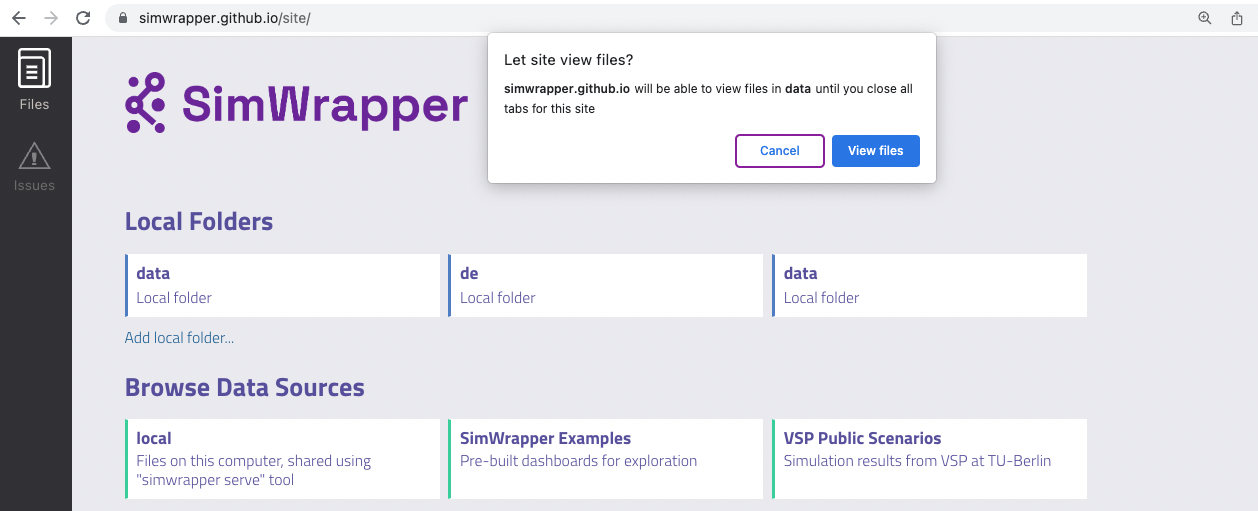
\includegraphics[width=0.8\linewidth]{chapters/31-simwrapper/images/chrome-access.png}
  \caption{Local file access security prompt on Google Chrome.}
  \label{fig:simwrapper-chrome}
\end{figure}


\hypertarget{simwrapper-cors}{%
\subsection{Accessing files from external websites: CORS}
\label{simwrapper-cors}}

Cross-origin resource sharing \gls{CORS} is a web technology which determines whether one website can retrieve content and assets from another website. Generally this is disallowed without explicit configuration and permission.

SimWrapper depends on the ability to retrieve files from external storage servers, so those servers must be configured to allow SimWrapper to access them.

In many cases this amounts to the file server requiring one additional line of configuration, for example the NGINX caching file server would require the following line,

\texttt{add\_header Access-Control-Allow-Origin "*";}

The asterisk "*" tells NGINX that all external websites can request files and the requests will be honored. The site administrator could be more specific and just authorize a list of SimWrapper websites instead; for example,

\texttt{add\_header Access-Control-Allow-Origin "simwrapper.github.io,vsp.berlin";}

CORS configuration can be much more complex than this, but this one line is usually sufficient. For much more detail on the CORS mechanism, see for example \url{https://developer.mozilla.org/en-US/docs/Web/HTTP/CORS}.


% ------------------------------------------------------------------------------------
% ## Converting purpose-built vizes into Generic Data Viewers
% ------------------------------------------------------------------------------------

\hypertarget{simwrapper-converting-purpose-built-visualizations-into-generic-data-viewers}{%
\section{Creating SimWrapper plugins from purpose-built visualizations}
\label{simwrapper-converting-purpose-built-visualizations-into-generic-data-viewers}}

The underlying infrastructure -- the build system, the user interaction libraries, and the choice of JavaScript component libraries -- was essentially complete after the PAVE, AVOEV, and COVID-Sim projects were operational. But the specific views imported from those project sites required a great deal of retooling to make them useful in a generic manner.

This section describes some of the most challenging aspects of this process of genericizing SimWrapper.

% ------------------------------------------------------------------------------------
% ### Link Viewer
% ------------------------------------------------------------------------------------

\hypertarget{simwrapper-link-viewer}{%
\subsection{Link viewer}\label{simwrapper-link-viewer}}

The link viewer was originally scoped to display link volumes only, such as a typical ``bandwidth plot'' commonly used in travel modeling. Even for PAVE this was shortsighted, as the project team quickly found other uses for the viewer such as link-based emissions.

Two major updates for SimWrapper are (1) the removal of the assumption that the data inputs will always have time period data in the columns followed by a ``grand total'' column; and (2) link colors and link bandwidths are now separately configurable.

An example is seen in Figure \ref{fig:simwrapper-network-links}. As is typical for road volume plots produced for transport planning, thicker lines indicate larger differences between scenarios, and red/blue colors are used for more and less traffic, respectively. User testing shows that a great deal more could still be done on these plots to meet user expectations. Data filters, automatic legends and configurable hovers are highly-requested enhancements, as well as a first-class ``difference mode''.

\begin{figure}[ht]
  \centering
  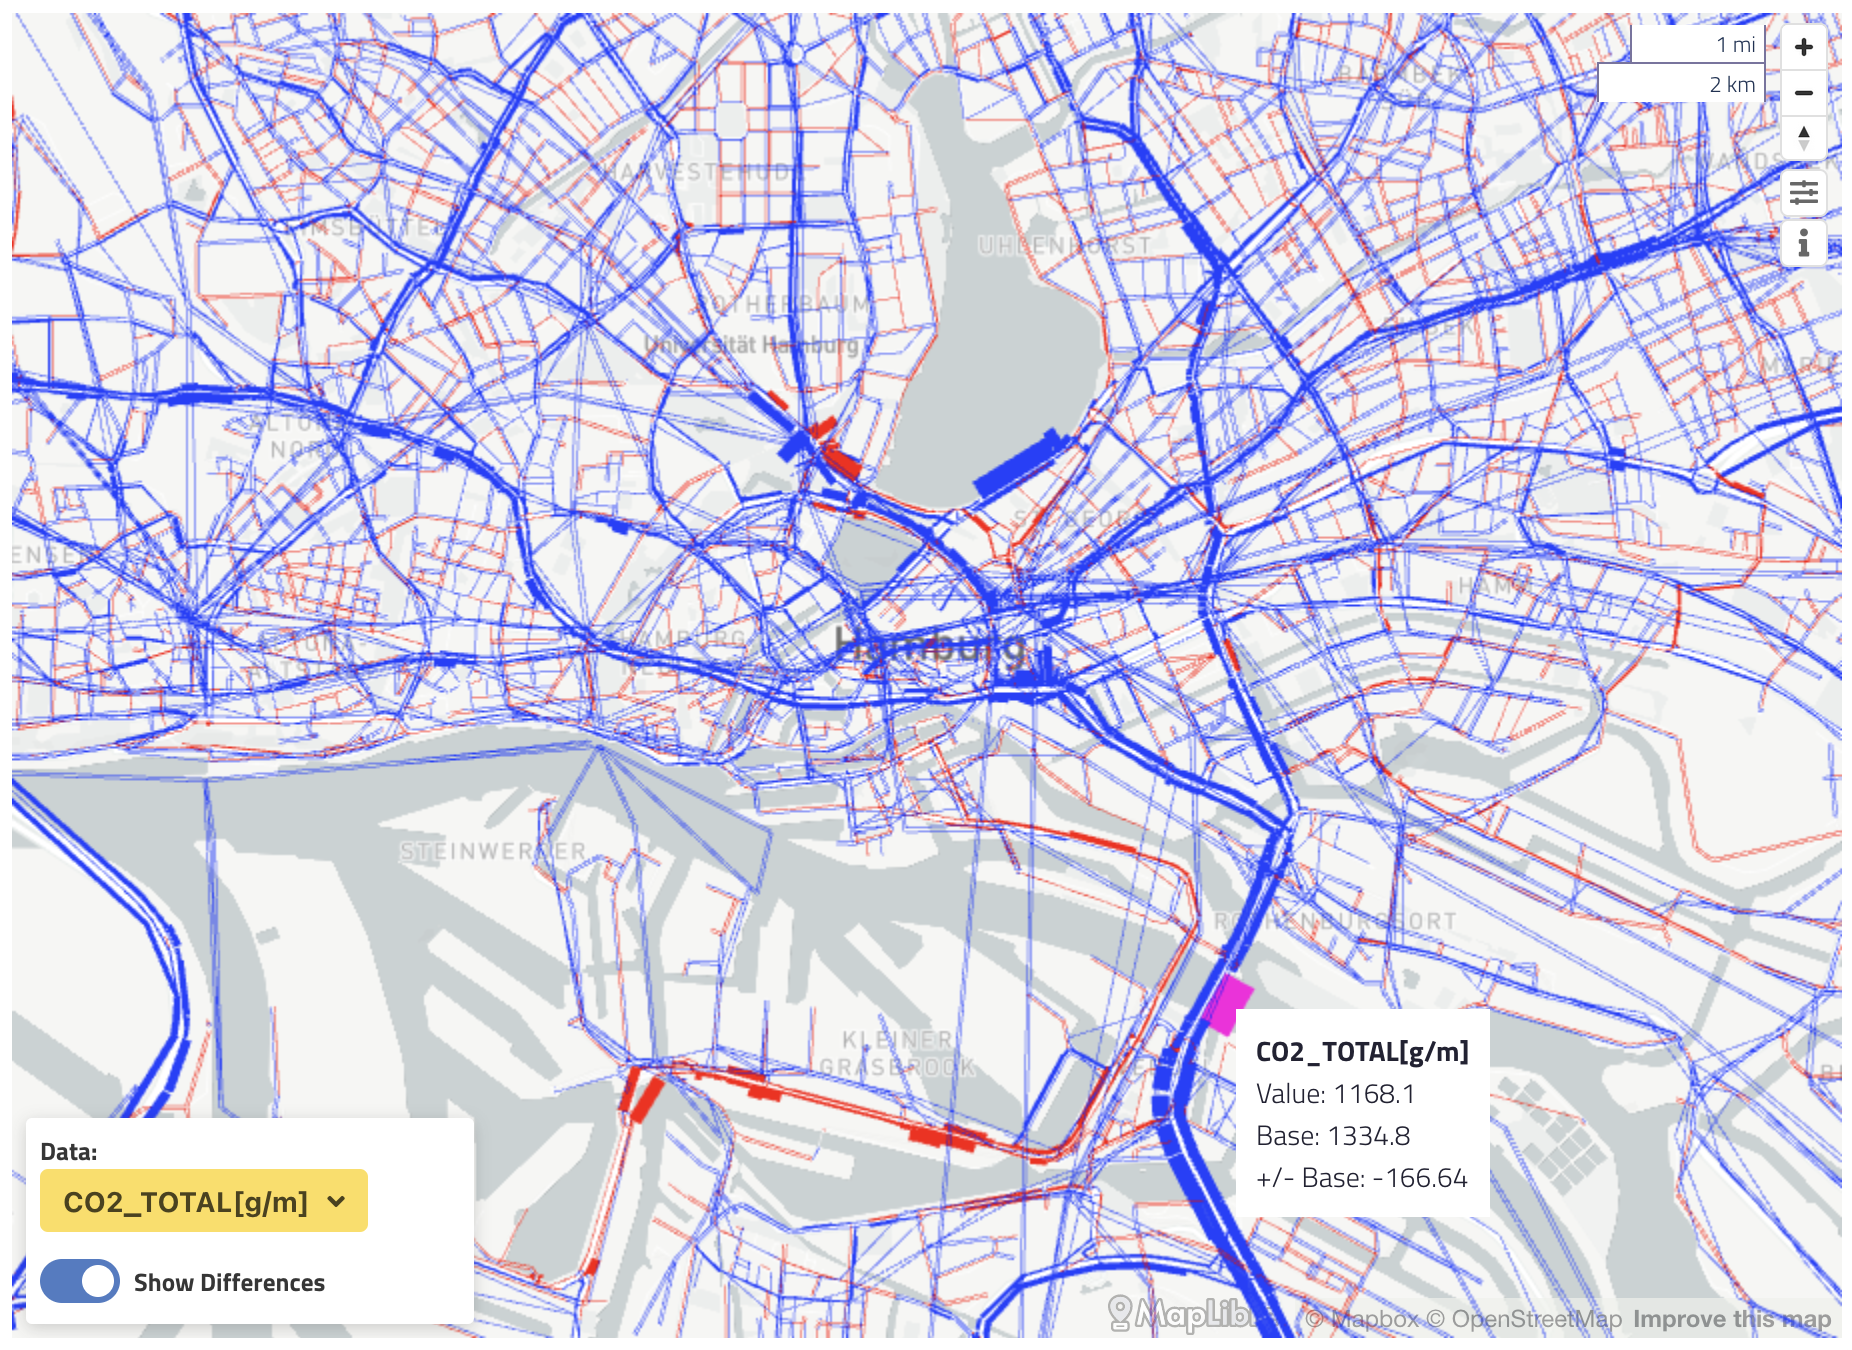
\includegraphics[width=0.7\linewidth]{chapters/31-simwrapper/images/network-links.png}
  \caption{Example network difference plot with user-configured colors and bandwidths for a Hamburg, Germany simulation comparison. Wider links represent larger differences; blue and red links depict positive and negative differences comparing two runs. }
  \label{fig:simwrapper-network-links}
\end{figure}

% ------------------------------------------------------------------------------------
% ### XY Data Plots
% ------------------------------------------------------------------------------------

\hypertarget{simwrapper-xy-hexagon-plots}{%
\subsection{XY hexagons plot}\label{simwrapper-xy-hexagon-plots}}

Even for transport simulations, not all data is link-based. Activity locations, home locations, pickups and dropoffs for transit and taxi modes, all have geographic coordinates associated with them but are not necessarily attached to specific road or transit links.

An additional visualization type, the ``XY Hexagons'' plot, depicts these types of data by aggregating them into user-definable hexagonal buckets. The number of points inside the hexagons corresponds to a color or height; this is user-configurable.

The default MATSim output \texttt{output\_trips.csv} includes this type of data, and is automatically viewable without any configuration at all if that standard file is present in a SimWrapper data folder.

Figure \ref{fig:simwrapper-xy-hexagons} shows a typical \texttt{output\_trips.csv} visualization using the XY Hexagons plot.

\begin{figure}[ht]
  \centering
  
\includegraphics[width=0.95\linewidth]{chapters/31-simwrapper/images/xy-hexagons.jpg}
  \caption{Example hexagon-based aggregation of standard MATSim output trips data. Flat and 3D visualizations are possible as shown. Color and height depict the aggregate total of trips originating from each area. }
  \label{fig:simwrapper-xy-hexagons}
\end{figure}

\hypertarget{simwrapper-xyt-plots}{%
\subsection{XY point plot}\label{simwrapper-xy-point-plots}}

Another X/Y data visualization type foregoes the aggregation of data rows into hexagons, and instead plots every point directly on the map, possibly by time of day. This plot is intended for point-based data such as emission measurements.

This is the first plugin to experiment with \emph{streaming the data file} while it is being loaded, instead of loading the entire dataset into memory, processing it in its entirety, and then producing the visualization. Instead, blocks of data are read from the CSV input file, the point data extracted, and then the memory holding those blocks is freed as new blocks are read. In this manner, datasets of up to 50 million rows are successfully displayed. This approach requires some new Web functionality that was not available before 2022 in all major browsers (the ability to stream so-called ``blob'' contents), and hints at some exciting possibilities for future enhancements for other large data file types.

Figure \ref{fig:simwrapper-xy-point-data} shows one example of point-based emission data that covers an area of Berlin. The points in this example are on a regular ten-meter grid and are so closely spaced that the individual points are difficult to discern. Smaller datasets with fewer points, or point data not on a grid, can also be visualized using this plugin.

\begin{figure}[ht]
  \centering
  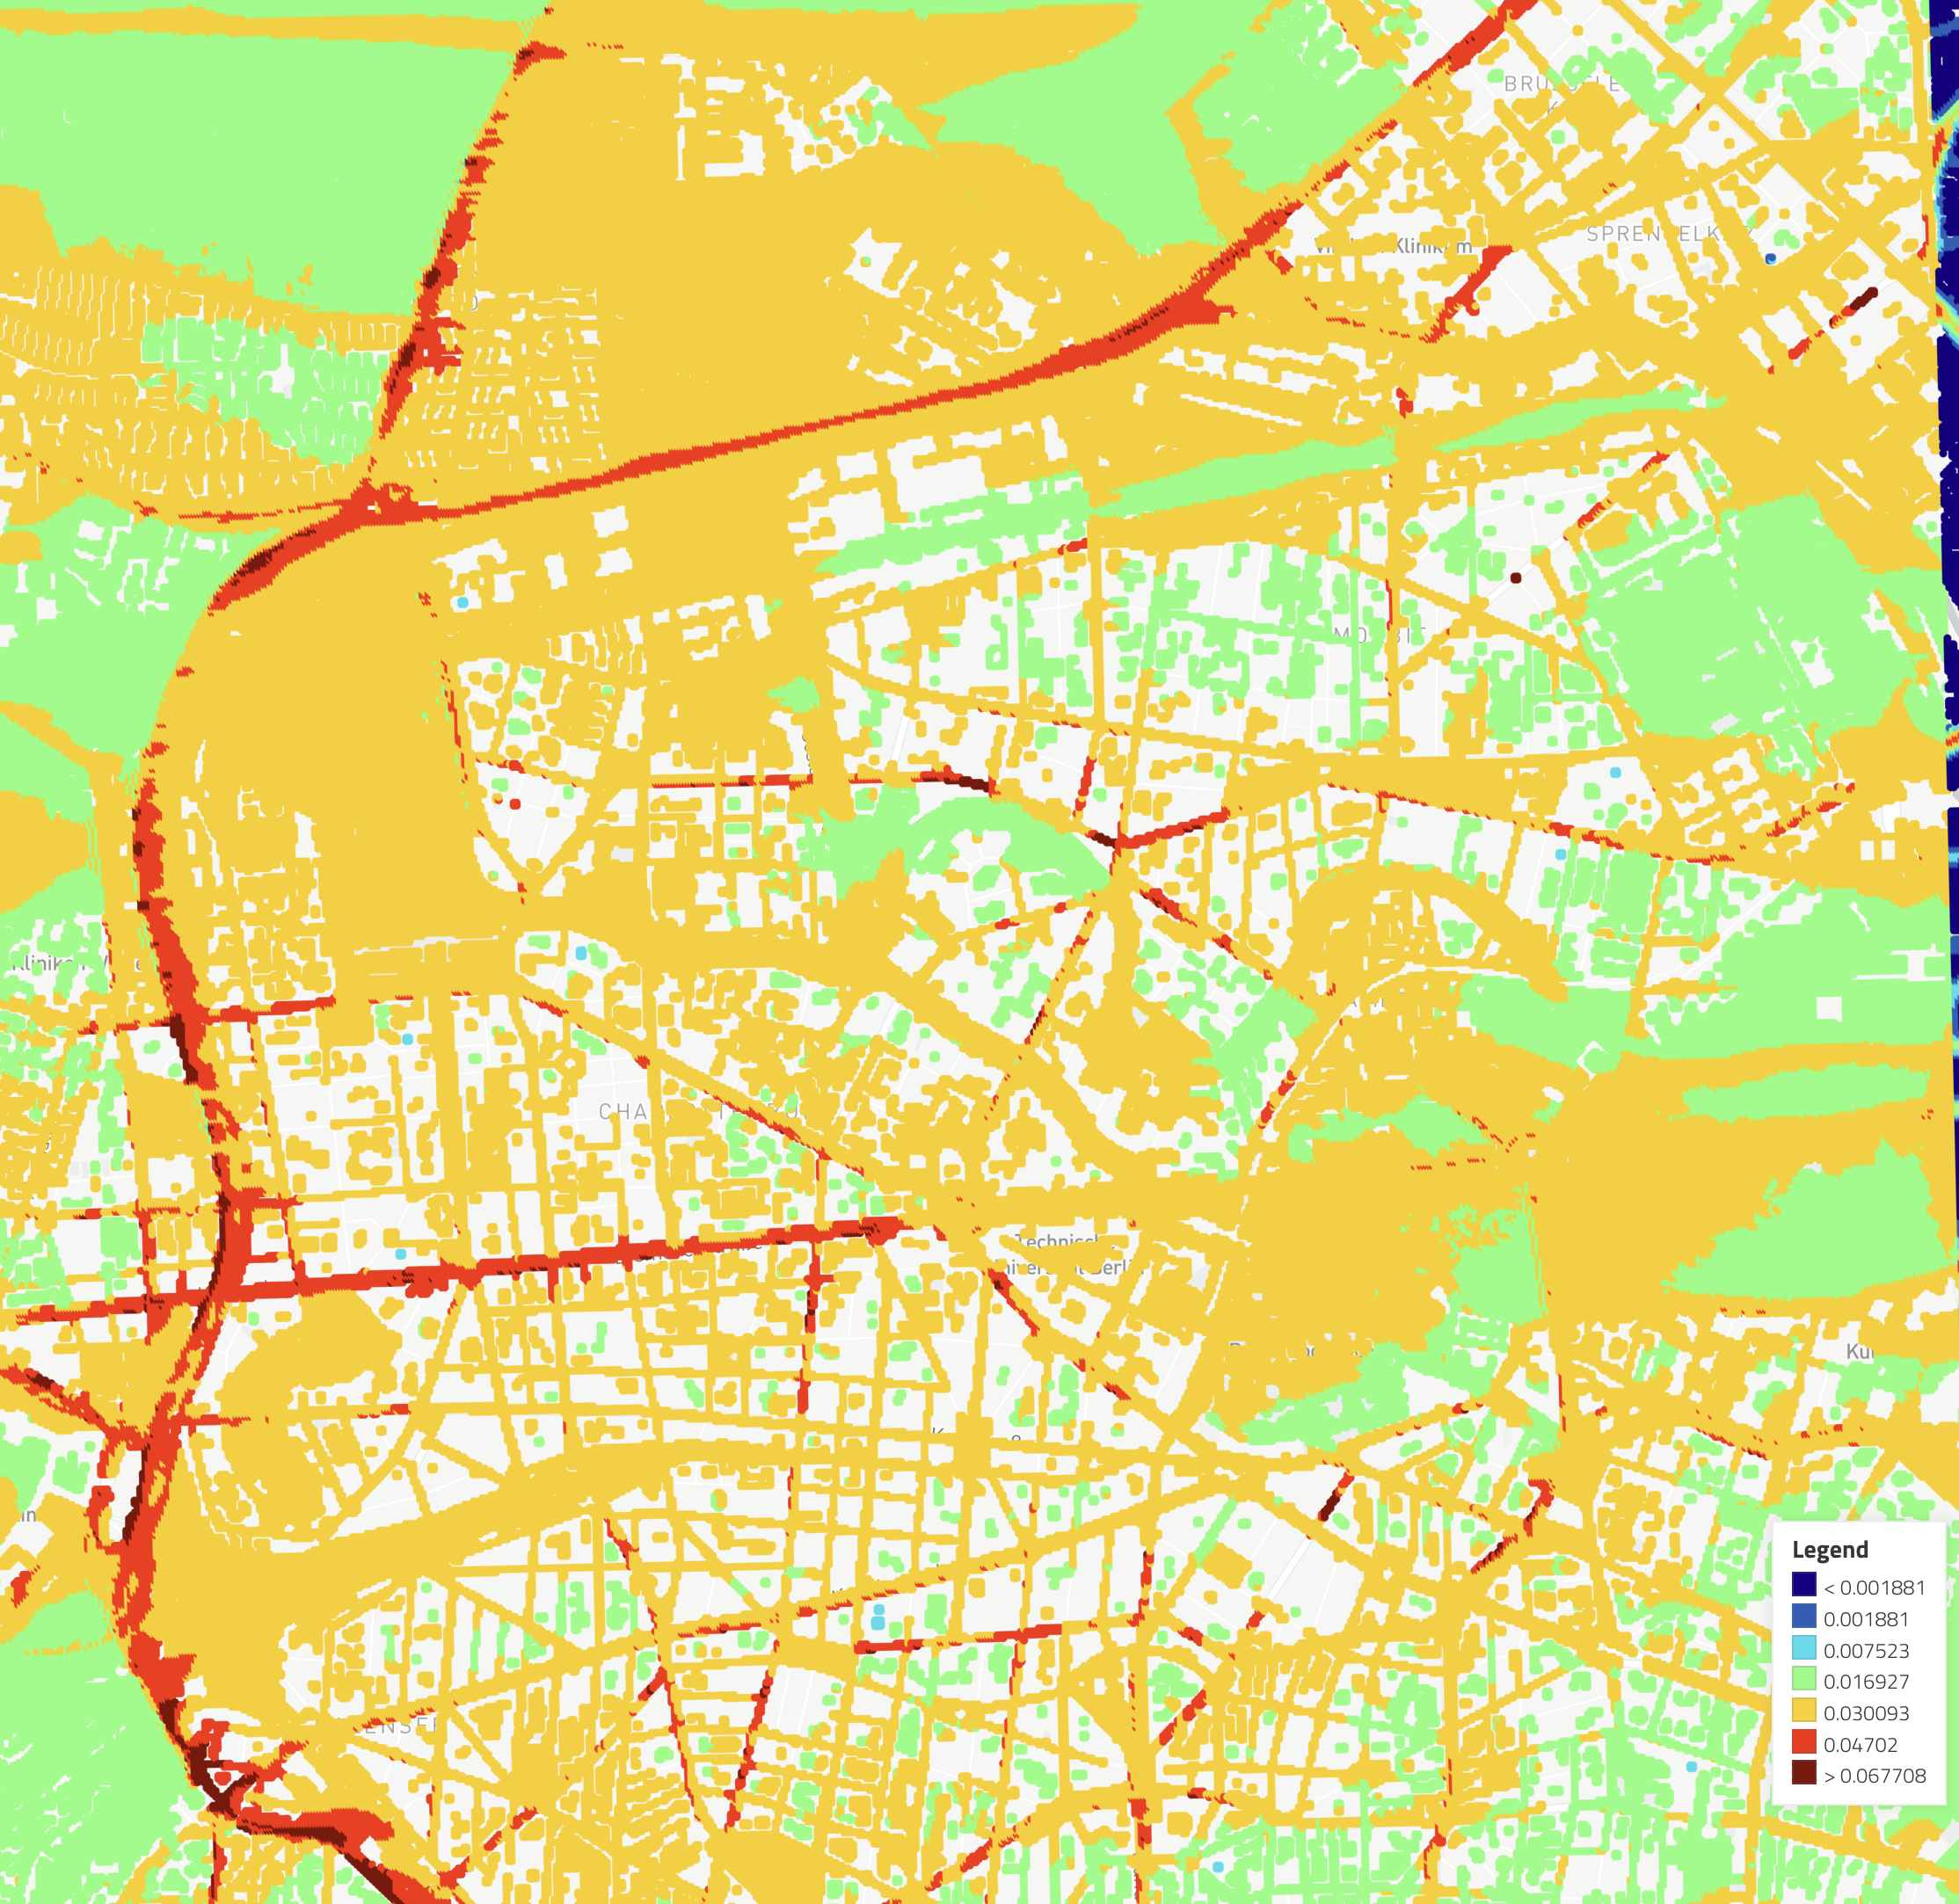
\includegraphics[width=0.6\linewidth]{chapters/31-simwrapper/images/xy-point-data.png}
  \caption{X/Y point data on a small regular grid, depicting emission values for an example Berlin microsimulation. The legend showing emission values is auto-generated by the visualization.}
  \label{fig:simwrapper-xy-point-data}
\end{figure}

% ------------------------------------------------------------------------------------
% ## Calculation Tables
% ------------------------------------------------------------------------------------

\hypertarget{simwrapper-calculation-tables}{%
\section{Calculation tables: providing top-line summary metrics}
\label{simwrapper-calculation-tables}}

Early in the development of SimWrapper, user feedback identified the need for reporting basic summary statistics and generating common aggregate values from model runs. These top-level summaries provide the first indication of useful results, such as overall mode share, average travel times, total emissions, and so forth. In addition, these measures are an excellent way to ``sanity-check'' a model run; in other words, to identify any obvious glaring errors in those topline numbers when compared to previously-established norms.

The first element needed is a straightforward way for users to specify the inputs, outputs, and formatting of calculation tables, compatible with the file-based configuration approaches already in use for the graphical visualizations. A second challenge is to formulate a clear and accurate scheme for specifying the needed calculations, including statistical transformations of the inputs such as counts, sums, and so on. Finally, the tool must perform those calculations in memory and produce the display the results.

These three elements are explored in order.

% ------------------------------------------------------------------------------------
% ### Calculation Table Config: Inputs, Files, Outputs
% ------------------------------------------------------------------------------------

\hypertarget{simwrapper-calculation-tables-definition}{%
\subsection{Specifying calculation table files, inputs, and outputs }\label{calculation-tables-definition}}

The most robust way to generate and display a table of numbers is by having the user develop their own post-processing scripts which output a simple CSV with the summary values and labels that they need. For this approach, nothing special is needed; whatever data analysis pipelines the analyst is already using are sufficient. Especially for more complex post-processing needs, using a high-quality platform such as Python or R is the recommended path.

For more simple summaries, SimWrapper includes a plugin that can extract and minimally process typical data files in CSV and XML formats. The need for this plugin is clear and based on the hesitancy of some analysts to write Python and R scripts (since MATSim simulation experts are generally far more familiar with Java programming than those languages). If all one needs is the sum of a column of values or the count of some event types, learning Python and debugging a Python script is perhaps overkill.

As the file-based YAML configuration paradigm for SimWrapper is at this point well-established, a new YAML configuration schema for table calculations is the most natural way to express these table definitions.

A new \texttt{table-*.yml} YAML schema containing four sections emerged from extensive iteration with users. The four required sections are:

\begin{itemize}

  \item \textbf{files}: The set of input file or files required for the table. These can be raw MATSim outputs or the results of any pre- or post-processing that has already occurred in the analyst data pipeline.

  \item \textbf{interactive input entries}: This is a list of user-editable entries that are visible on interactive web form. Some calculations benefit from having a variable input that the website user can specify; imagine fuel cost per liter, or number of vehicles in a taxi fleet. Each of these entries can have a default value.

  \item \textbf{calculations}: An ordered list of mathematical calculations to be performed. Variables, data columns, and interactive elements specified above are combined in equations as needed. This is described in detail below.

  \item \textbf{outputs}: The final table entries are specified with formatting and labels.

\end{itemize}

Three of the four sections --- \emph{files}, \emph{interactive entries}, and \emph{outputs} --- are trivially specified and do not require extensive exposition here: they are straightforward definitions of file names, titles, and formatting directives. These are well-documented in the documentation available on the SimWrapper website (\cite{SimWrapperWebsite}).

The calculations are more interesting and are explored next.

% ------------------------------------------------------------------------------------
% ### Calculation Table DSL: Specifying the Equations
% ------------------------------------------------------------------------------------
\hypertarget{calculation-tables-dsl}{%
\subsection{Specifying calculations using a domain-specific language}\label{calculation-tables-dsl}}

The final and most important piece of specifying calculations is devising the equation format to be used in the YAML configuration, which brings together the interactive value inputs, the required input files, data columns in those files (and any data manipulations thereon), and combines them all in understandable algebraic equations that can be solved by the tool.

This is more akin to a \gls{DSL} than a configuration file.

\cite{Visser2008} defines a domain-specific language as follows, ``A domain-specific language (DSL) is a high-level software implementation language that supports concepts and abstractions that are related to a particular (application) domain.'' Visser explains further that a DSL is in essence ``the encapsulation of design and implementation knowledge from a particular application or technical domain. The commonalities of the domain are implemented directly in a conventional programming language or indirectly in code generation templates, while the variability is configurable by the application developer through some configuration interface.''

This is precisely what the YAML calculation definitions set out to do: allow a user who is an expert in the dataset and the needed transformations for a particular metric, to define that in a manner that does not require them to write a data analysis script in a full-fledged programming language such as R or Python.

The DSL devised for the SimWrapper table plugin has the following components. See the plugin documentation on the SimWrapper website for full examples.

\textbf{Calculation scripts.} Each table definition has a \emph{calculation} section which is a list of mathematical calculations, evaluated in order from top to bottom. Each line defines a value for a variable name, and subsequent lines can use that calculated value. In this way, fairly complex calculations can defined over several lines.

\textbf{Writing equations.} The NPM library \emph{nerdamer} provides a robust and well-tested equation parsing library. This library calculates the value of equations written in typical mathematical notation, e.g. \texttt{100 + 0.25*6000}. The plugin replaces variable names with actual numerical values, so that \emph{nerdamer} can actually perform the math.

\textbf{Selecting data from the inputs.} Data input files are defined in the \emph{files} section, supporting both CSV and XML array objects. In the calculation section, columns of data are selected using a ``file.column'' notation, e.g. \texttt{emissions.co2} and so on.

\textbf{Statistical transformations.} Standard statistical reduction functions can be specified: \emph{@sum, @count, @max, @min} are supported and are applied across an entire column of values.

\textbf{Filtering.} Logical filters can be applied using a \emph{@filter(variable < == > value)} function.

Figure \ref{fig:simwrapper-calculation-table} shows an example of calculation equations.

\begin{figure}[ht]
  \centering
  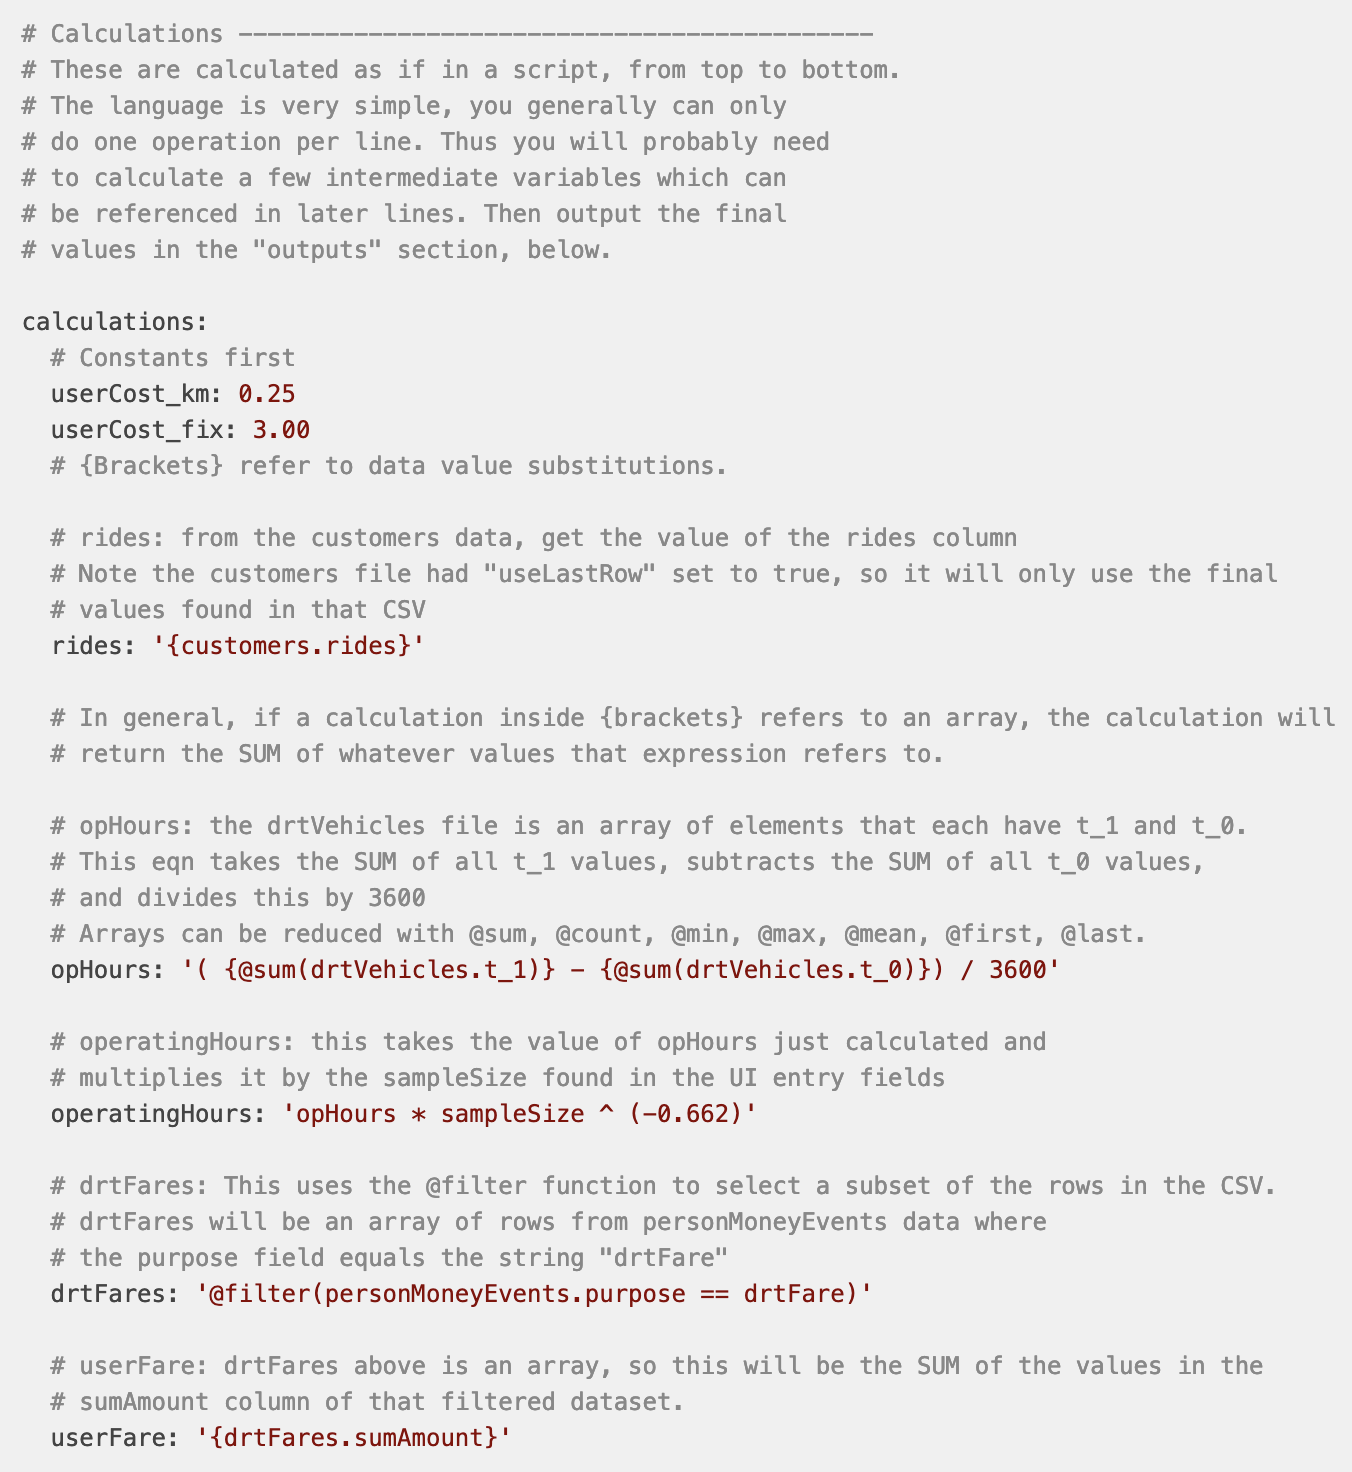
\includegraphics[width=0.7\linewidth]{chapters/31-simwrapper/images/calculation-table.png}
  \caption{Calculation plugin specifications for an example table. This shows a sample calculation section with several file and variable references and statistical transformations.}
  \label{fig:simwrapper-calculation-table}
\end{figure}


% ------------------------------------------------------------------------------------
% ## Dashboards
% ------------------------------------------------------------------------------------

\hypertarget{simwrapper-dashboards}{%
\section{Dashboards: combining visualizations to support decisionmaking}\label{simwrapper-dashboards}}

A dashboard is a page laid out with multiple charts, plots, and visualizations all on one canvas. The layout is, as with everything SimWrapper, defined in a YAML file that contains the types of plots, the dashboard layout definition, and their configuration parameters, all in one place.

\begin{figure}[ht]
  \centering
  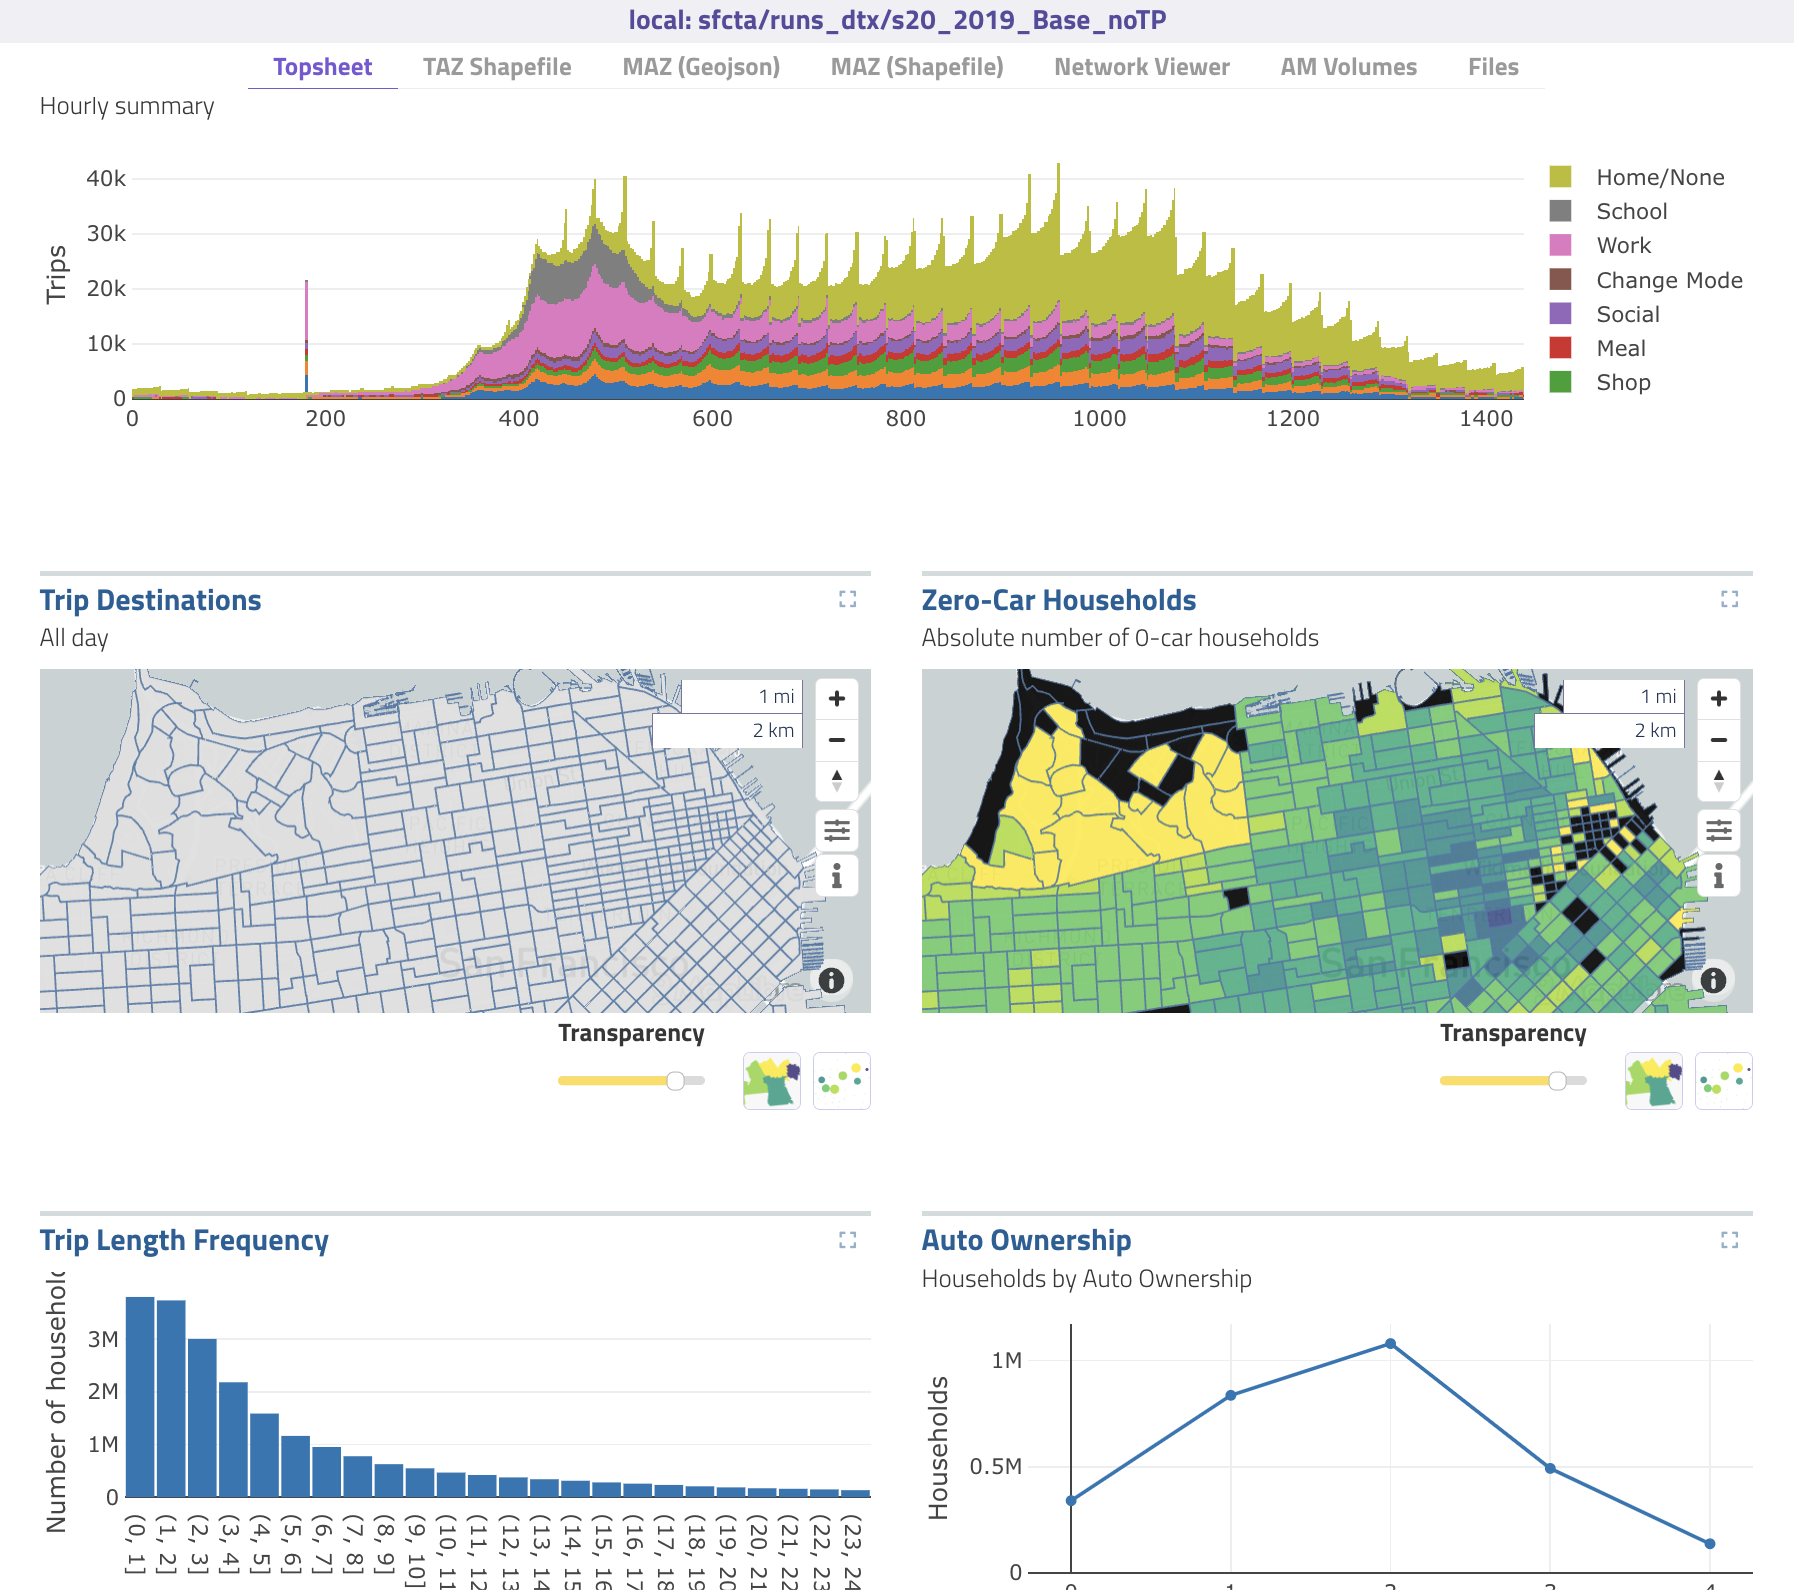
\includegraphics[width=0.7\linewidth]{chapters/31-simwrapper/images/dashboard.png}
  \caption{Dashboards often show several views or at-a-glance summary metrics on one pane.}
  \label{fig:simwrapper-dashboard}
\end{figure}


Figure \ref{fig:simwrapper-dashboard} shows a simple dashboard with multiple tabs organizing different topical areas (topsheet, volumes, zonal summaries). In SimWrapper, a folder containing any number of \texttt{dashboard-*} YAML files will display the dashboards in addition to the usual folder browser view. When multiple dashboard YAML files exist, they will be shown as multiple navigation tabs on the page as in the figure.

\begin{itemize}
\item
  The layout consists of a set of named \textbf{rows}. The row name
  themselves are not shown anywhere, they are there to help organize the
  file.
\item
  Each \texttt{row} consists of a list of view panels. By default, all
  panels in the row will be laid out horizontally from left to right,
  in equal widths. This can be configured.
\item
  Finally, each element in a row has specific properties that define the
  actual chart or visualization that will be displayed.

  \begin{itemize}
  \item
    \textbf{type} The chart or plot type, e.g.~\texttt{pie},
    \texttt{bar}, \texttt{flowmap}, etc. See the individual chart docs
    for all available plots.
  \item
    \textbf{title} The name of the plot
  \item
    \textbf{description} A brief description (optional)
  \item
    \textbf{width} One can set \emph{relative widths} by adding the
    \texttt{width:\ {[}number{]}} property. Charts have a default width
    of 1. Thus in a row with 3 charts, if the width of the first object
    is 2, then {[}2+1+1{]} means the first object fills 50\% of the row,
    and the remaining two objects fill 25\% each. (optional)
  \item
    \textbf{props} The set of configuration settings for this chart,
    such as the dataset to load, which columns to use, etc.
  \item
    \emph{The chart type determines the set of valid properties!}
  \end{itemize}
\end{itemize}

This system of defining dashboards in configuration has been used to great effect in many internal studies, some examples are shown in \ref{ch:simwrapper-sites}.

% ------------------------------------------------------------------------------------

\hypertarget{simwrapper-project-level-configuration}{%
\subsection{Project-level configuration}\label{project-level-configuration}}

Users often express interest in setting up standardized output summaries in the form of dashboards or consistent visualizations across simulation outputs, and to use those for every model run for that project.

SimWrapper handles this use case by recognizing a \texttt{simwrapper} or \texttt{.simwrapper} folder in (or above) the output data folders. This folder contains any common configuration files, whether they be dashboard layouts, individual visualization parameters, or table calculation definitions. For all project folders in the same parent folder and for all child folders as well, SimWrapper behaves as if these configuration files are present in the current folder. In this way, departmental standard dashboards are merged with project- and simulation-specific configurations as needed.

% ------------------------------------------------------------------------------------

\hypertarget{simwrapper-discussion}{%
\section{Discussion}\label{simwrapper-discussion}}

SimWrapper has been live since mid-2022 and over time has acquired data visualization plugins for most of the types of data that transport planners would like to see: link data, point data, statistical charts and plots, and aggregate data views of many types. Furthermore these views can be collated into cohesive dashboards for specific runs and defined at a project-level.

User feedback internally at VSP has been positive, acknowledging that the platform is a work in progress and there are continuous updates, bugfixes, and changes happening in real time.

Staff at VSP are now building a standard MATSim results dashboard based on SimWrapper. This dashboard is expected to traverse several navigation tabs which collate the summaries into topical areas, such as Overview, Trips, Public Transport, Emissions, Stuck Agents, and so on.

Outside of VSP, SimWrapper has also now been picked up by a small handful of public agencies across the globe.

The file-based nature of SimWrapper is a strength, in that it matches the file-based reality of the simulation models that it is most often paired with. But this is also a challenge, because large file sizes are a constant source of problems. Significant time has been invested in hyper-optimizing memory usage, something that might not be necessary in a server/database based system in which only portions of data are ingested at a time. But as a counterpoint, SimWrapper requires no database server so is very easy for end users to just start using without worrying too much about initial setup and configuration.

\hypertarget{simwrapper-tool-comparison}{%
\subsection{Comparison to other tools and approaches}\label{simwrapper-tool-comparison}}

\textbf{R/Shiny dashboards.} The R statistical analysis platform offers an open-source dashboard tool called ``Shiny'' that is popular and comprehensive\footnote{Shiny is available at \url{https://www.rstudio.com/products/shiny/}}. Shiny requires an R server running either locally or from a cloud service. The interactivity and consistent look and feel of Shiny dashboards is compelling. Shiny does not know anything about MATSim so simulation outputs require extensive postprocessing to be included in a dashboard. Advanced Deck.gl visualizations can be embedded in Shiny, but the typically large MATSim datasets are quite slow to load and render. SimWrapper is extensively optimized to load and display MATSim datasets quickly. Nonetheless Shiny provides a nice alternative for teams that already have experience with R and wish to extend that platform instead of learning and adapting to SimWrapper's unique approach.

\textbf{Python/Dash dashboards.} There are numerous dashboarding tools available in the Python language ecosystem, such as the popular "Dash" tool \footnote{Python Dash is available at \url{https://dash.plotly.com/}}. Like R/Shiny above, these tools are all nice alternatives to SimWrapper for teams which have already invested in Python, and similar to Shiny, these tools require a Python server running either locally or in a cloud service. The plethora of options in the Python ecosystem make it a bit difficult to know which dashboard tool is the best fit, Dash seems to be popular and comprehensive.

\textbf{Jupyter notebooks.} Online "notebooks" such as Jupyter\footnote{Jupyter is availabe at \url{https://jupyter.org/}} provide a web-based interactive development option for analysts. An advantage of notebooks is that they allow researchers to combine code, data, and exposition in one top-down lab-style document. In general the very technical content of these lab-style notebooks is not appropriate for non-scientific audiences. These notebooks are, however, very useful for internal teams for tasks such as scenario comparison and model debugging. Again, all notebook systems require a server running either locally or from a cloud provider.

\textbf{Commercial offerings: PTV and Simunto.} There are many commercial offerings for online dashboard tools. Just limiting the comparison to a few well-known transport simulation offerings, both PTV and Simunto offer cloud dashboard products for a monthly fee (at the time of writing the Simunto product is still in beta). For teams that are already invested in PTV products this can be a very easy and frictionless way to publish summaries online. The feature set of ``PTV Visum Publisher'' is in general smaller that what SimWrapper provides, but the user interface and product polish are quite high in comparison. The PTV product allows multi-layer map visualizations, something that SimWrapper currently does not allow (but is under consideration for future development).

In summary, the featureset of SimWrapper is useful enough for practitioners and unique enough compared to other tools, that the user base continues to grow as of this writing.

% ------------------------------------------------------------------------------------

\hypertarget{simwrapper-summary}{%
\section{Summary}\label{simwrapper-summary}}

This chapter describes SimWrapper, a general data visualization platform that is custom-designed to meet the needs of transport simulation experts. The platform is live on the web and now has a small set of users from many cities worldwide. The success of the platform so far is encouraging: there does seem to be a desire for the ability to rapidly produce web-based data visualizations and dashboards for debugging, sharing, and publicizing microsimulation results.

Many different data visualization types are available in SimWrapper, including most of the types of charts and maps that a transport planner would be interested in: link data, point data, aggregate data maps, thematic maps, and myriad statistical charts and plots can all be displayed alone or in custom-curated dashboards. It is possible to view local data and also to publish these dashboards online or on internal shared servers.

Limitations of the platform exist; as there is no database or server back-end, the size of data files and the speed at which those data files can be ingested by a local web browser are limiting factors. Despite this, the functionality has proven useful.

Based on the initial success and use of SimWrapper, further development will continue to add additional visualization types, and like any software project, to improve performance and fix bugs.
